%!TEX root = /Users/ego/Boulot/Alterqcm/doc/doc_aq-main.tex
\section{Options globales de l'environnement  \tkzname{alterqcm}}

\subsection{\tkzname{lq} : modification de la largeur de la première colonne }
\IoptEnv{alterqcm}{lq}

\begin{alterqcm}[long,lq=110mm]
\AQquestion{Parmi les propositions suivantes, quelle est celle qui permet %
 d'affirmer que la fonction exponentielle  admet pour asymptote %
  la droite d'équation $y = 0$ ?}
{{$\displaystyle\lim_{x \to +\infty} \text{e}^x = + \infty$},
{$\displaystyle\lim_{x \to -\infty} \text{e}^x = 0$},
{$\displaystyle\lim_{x \to +\infty} \dfrac{\text{e}^x}{x} = + \infty$}}

\AQquestion{exp$(\ln x) = x$ pour tout $x$ appartenant à }
{{$\mathbb{R}$},
{$\big]0~;~+ \infty\big[$},
{$\big[0~;~+\infty\big[$}
}
\end{alterqcm}

\medskip
Voyons le code nécessaire pour obtenir ce tableau. Il faut  placer
\tkzcname{usepackage\{alterqcm\}} dans le préambule. Il faut remarquer que seule la largeur de la colonne des questions est fournie |lq=100mm| et que cela est optionnel. Le nombre des propositions est ici \textbf{3} mais il peut varier d'une question à l'autre.

\begin{tkzexample}[code only,small]
 \begin{alterqcm}[long,lq=110mm]
  \AQquestion{Parmi les propositions suivantes, quelle est celle qui permet %
  d'affirmer que la fonction exponentielle  admet pour asymptote %
    la droite d'équation $y = 0$ ?}
  {{$\displaystyle\lim_{x \to +\infty} \text{e}^x = + \infty$},
  {$\displaystyle\lim_{x \to -\infty} \text{e}^x = 0$},
  {$\displaystyle\lim_{x \to +\infty} \dfrac{\text{e}^x}{x} = + \infty$}}
  
  \AQquestion[]{exp$(\ln x) = x$ pour tout $x$ appartenant à }
  {{$\mathbb{R}$},
  {$\big]0~;~+ \infty\big[$},
  {$\big[0~;~+\infty\big[$}
  }
  \end{alterqcm}\end{tkzexample}



\subsection{\tkzname{pq} : utilisation globale }
 \IoptEnv{alterqcm}{pq}  

Cette fois, il est nécessaire de déplacer plusieurs questions, j'ai placé un |pq=2mm| globalement c'est à dire comme ceci :\tkzcname{begin\{alterqcm\}[lq=85mm,pq=2mm]}. \textbf{Toutes} les questions sont affectées par cette option mais certaines questions  étaient bien placées et doivent le rester, aussi localement je leur redonne un |pq=0mm|.

\medskip
\begin{alterqcm}[lq=85mm,pq=2mm]
\AQquestion{Soit une série statistique à deux variables. Les valeurs de $x$ sont 1, 2, 5, 7, 11, 13 et une équation de la droite de régression de $y$ en $x$ par la moindres carrés est $y = 1,35x +22,8$. Les coordonnées du point moyen sont :}
{{$(6,5;30,575)$},
{$(32,575 ; 6,5)$},
{$(6,5 ; 31,575)$}}

\AQquestion{Pour tout réel $x$, le nombre \[\dfrac{\text{e}^x - 1}{\text{e}^x + 2}\hskip12pt \text{égal à :} \] }
{{$-\dfrac{1}{2}$},
{$\dfrac{\text{e}^{-x} - 1}{\text{e}^{-x} + 2}$},
{$\dfrac{1 - \text{e}^{-x}}{1 + 2\text{e}^{-x}}$}
}
\AQquestion{On pose I $= \displaystyle\int_{\ln 2}^{\ln 3} \dfrac{1}{\text{e}^x - 1}\,\text{d}x$ et J $ = \displaystyle\int_{\ln 2}^{\ln 3} \dfrac{\text{e}^x}{\text{e}^x - 1}\,\text{d}x$ \\ alors le nombre  I $-$ J est égal à}
{{$\ln \dfrac{2}{3}$},
{$\ln \dfrac{3}{2}$},
{$\dfrac{3}{2}$}
}
\end{alterqcm}

\begin{tkzexample}[code only,small]
 \begin{alterqcm}[lq=85mm,pq=2mm]
 \AQquestion{Pour tout réel $x$, le nombre \[\dfrac{\text{e}^x - 1}
 {\text{e}^x + 2}\hskip12pt \text{égal à :} \] }
 {{$-\dfrac{1}{2}$},
 {$\dfrac{\text{e}^{-x} - 1}{\text{e}^{-x} + 2}$},
 {$\dfrac{1 - \text{e}^{-x}}{1 + 2\text{e}^{-x}}$}}
 \end{alterqcm}
\end{tkzexample}


\subsection{\tkzname{VF} : Vrai ou Faux}
\IoptEnv{alterqcm}{VF}
Les propositions ne sont que  deux et le candidat doit choisir entre \textbf{Vrai} ou \textbf{Faux}. Cette fois, la syntaxe est allégée. Il n'est plus nécessaire d'écrire la liste des propositions et  il suffit de positionner \tkzname{VF}  en plaçant dans les options   \tkzname{$VF$}.

 
\begin{minipage}[t][][b]{.45\linewidth}
Soit $f$ une fonction définie et dérivable sur l'intervalle $\big[-3~;~+\infty\big[$, croissante sur les intervalles $\big[-3~;~-1\big]$ et $\big[2~;~+\infty\big[$ et décroissante sur l'intervalle $\big[-1~;~2\big]$.

 On note $f'$ sa fonction dérivée sur l'intervalle $[-3~;~+\infty[$.

La courbe $\Gamma$ représentative de la fonction $f$ est tracée ci-dessous dans un repère orthogonal $\big(O,~\vec{\imath},~\vec{\jmath}\big)$.

Elle passe par le point A$(-3~;~0)$ et admet pour asymptote la droite $\Delta$ d'équation $y =  2x -5$.
\end{minipage}
\hfill
\begin{minipage}[t][][b]{.45\linewidth}
\null
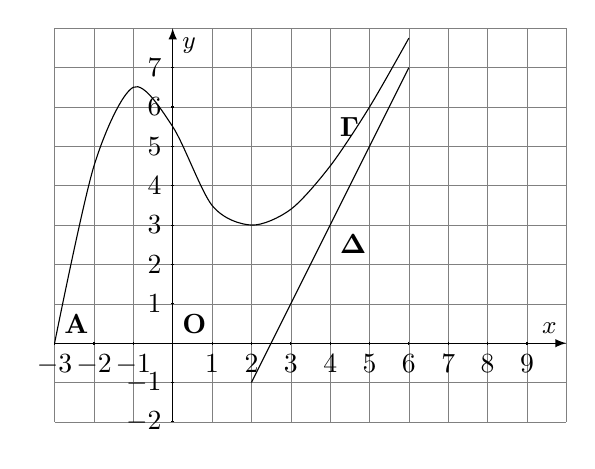
\begin{tikzpicture}[scale=0.5,>=latex]
 \draw[very thin,color=gray] (-3,-2) grid (10,8);
 \draw[->] (-3,0) -- (10,0) node[above left] {\small $x$};
 \foreach \x in {-3,-2,-1,1,2,...,9}
    \draw[shift={(\x,0)}] (0pt,1pt) -- (0pt,-1pt)node[below] { $\x$};
 \draw[->] (0,-2) -- (0,8) node[below right] {\small $y$};
 \foreach \y/\ytext in {-2,-1,1,2,...,7}
    \draw[shift={(0,\y)}] (1pt,0pt) -- (-1pt,0pt) node[left] { $\y$};
 \draw (2,-1) -- (6,7);
 \node[above right] at (-3,0) {\textbf{A}};
 \node[above right] at (0,0) {\textbf{O}};
 \node[below right] at (4,3) {$\mathbf{\Delta}$};
 \node[above right] at (4,5) {$\mathbf{\Gamma}$};
 \draw plot[smooth] coordinates{%
 (-3,0)(-2,4.5)(-1,6.5)(0,5.5)(1,3.5)(2,3)(3,3.4)(4,4.5)(5,6)(6,7.75)};
\end{tikzpicture}
\end{minipage}
                     

\begin{alterqcm}[VF,lq=125mm]
 \AQquestion{Pour tout $x \in ]-3~;~2],~f'(x) \geqslant 0$.}
 \AQquestion{La fonction $F$ présente un maximum en $2$}
 \AQquestion{$\displaystyle\int_{0}^2 f'(x)\,\text{d}x = - 2$}
\end{alterqcm}

\begin{tkzexample}[code only, small]
 \begin{minipage}[t][][b]{.45\linewidth}
  Soit $f$ une fonction définie et dérivable sur l'intervalle $\big[-3~;~+\infty\big[$,
   croissante sur les intervalles $\big[-3~;~-1\big]$ et $\big[2~;~+\infty\big[$
   et décroissante sur l'intervalle $\big[-1~;~2\big]$.
  
   On note $f'$ sa fonction dérivée sur l'intervalle $[-3~;~+\infty[$.
  
  La courbe $\Gamma$ représentative de la fonction $f$ est tracée ci-dessous
   dans un repère orthogonal $\big(O,~\vec{\imath},~\vec{\jmath}\big)$.
  
  Elle passe par le point A$(-3~;~0)$ et admet pour asymptote la droite
  $\Delta$ d'équation $y =  2x -5$.
 \end{minipage}
 \begin{minipage}[t][][b]{.45\linewidth}
 \null
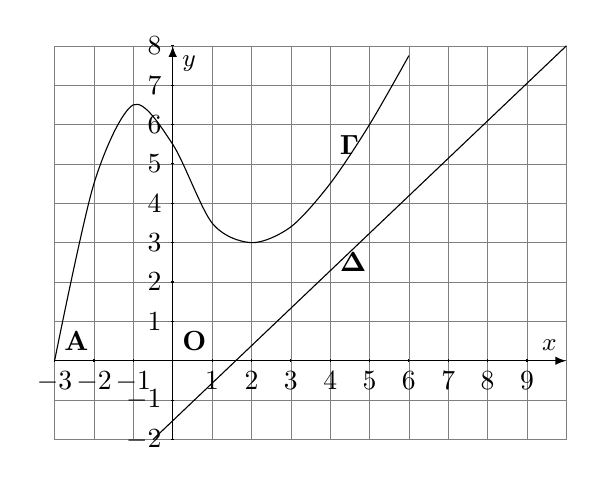
\begin{tikzpicture}[scale=0.5,>=latex]
  \draw[very thin,color=gray] (-3,-2) grid (10,8);
  \draw[->] (-3,0) -- (10,0) node[above left] {\small $x$};
  \foreach \x in {-3,-2,-1,1,2,...,9}
     \draw[shift={(\x,0)}] (0pt,1pt) -- (0pt,-1pt)node[below] { $\x$};
  \draw[->] (0,-2) -- (0,8) node[below right] {\small $y$};
  \foreach \y/\ytext in {-2,-1,1,2,...,8}
     \draw[shift={(0,\y)}] (1pt,0pt) -- (-1pt,0pt) node[left] { $\y$};
  \draw (-0.5,-2) -- (10,8);
  \node[above right] at (-3,0) {\textbf{A}};
  \node[above right] at (0,0) {\textbf{O}};
  \node[below right] at (4,3) {$\mathbf{\Delta}$};
  \node[above right] at (4,5) {$\mathbf{\Gamma}$};
  \draw plot[smooth] coordinates{%
  (-3,0)(-2,4.5)(-1,6.5)(0,5.5)(1,3.5)(2,3)(3,3.4)(4,4.5)(5,6)(6,7.75)};
 \end{tikzpicture}
 \end{minipage}
 \begin{alterqcm}[VF,lq=125mm]
   \AQquestion{Pour tout $x \in ]-\infty~;~2],~f'(x) \geqslant 0$.}
   \AQquestion{La fonction $F$ présente un maximum en $2$}
   \AQquestion{$\displaystyle\int_{0}^2 f'(x)\:\text{d}x = - 2$}
 \end{alterqcm}
\end{tkzexample}

\subsection{\tkzname{symb} : modification du symbole } 
\IoptEnv{alterqcm}{symb}

 Si vos fontes ne possèdent pas le symbole |$\square$| ou encore |$\blacksquare$| vous pouvez utiliser celui fourni par le package ou bien en créer un vous même. \tkzcname{altersquare}, \tkzcname{dingsquare} et \tkzcname{dingchecksquare} sont fournies par alterqcm.
 Voici comment sont définies ces macros.
 
\begin{tkzexample}[code only,small]
 \newcommand*{\altersquare}{\vbox{\hrule\hbox to 6pt%
 {\vrule height 5.2pt \hfil\vrule}\hrule}}\end{tkzexample}

\medskip on obtient \altersquare\ ou bien encore :

\begin{tkzexample}[code only,small]
 \newcommand*{\dingsquare}{\ding{114}} \end{tkzexample}

\medskip ce qui donne \dingsquare\ et enfin pour remplacer |$\blacksquare$| 

\begin{tkzexample}[code only,small]
 \newcommand*{\dingchecksquare}{\mbox{\ding{114}%
 \hspace{-.7em}\raisebox{.2ex}[1ex]{\ding{51}}}} \end{tkzexample}

\medskip Soit \dingchecksquare\ comme résultat. 


\begin{tkzexample}[code only,small] 

 \begin{alterqcm}[lq=90mm,symb=\altersquare]
 ... \end{alterqcm}\end{tkzexample}

\medskip
Exemple complet :

\medskip
\begin{tkzexample}[vbox]
 \begin{alterqcm}[VF,lq=125mm,symb    = \dingsquare]
 \AQquestion{Pour tout $x \in ]-3~;~2],~f'(x) \geqslant 0$.}
 \AQquestion{La fonction $F$ présente un maximum en $2$}
 \AQquestion{$\displaystyle\int_{0}^2 f'(x)\:\text{d}x = - 2$}
 \end{alterqcm}\end{tkzexample}
  

\subsection{\tkzname{pre, bonus, malus} : présentation automatique }
\IoptEnv{alterqcm}{pre}\IoptEnv{alterqcm}{bonus}\IoptEnv{alterqcm}{malus}
Comme vous pouvez le constatez ci-dessous, une présentation est donnée de l'exercice avec le barème.

\bigskip
\begin{minipage}[c][][t]{.45\linewidth}
\begin{tkzexample}[code only,small]
  \begin{alterqcm}[lq=6cm,pre=true,%
                   bonus=1,malus={0,5}]
  \AQquestion{Question}
  {{Proposition 1},
   {Proposition 2}}
  \end{alterqcm}\end{tkzexample}
\end{minipage}\hfill
\begin{minipage}[c][][t]{.45\linewidth}
  \begin{alterqcm}[lq=3cm,pre=true,
                   bonus=1,malus={0,5}]
  \AQquestion{Question}
  {{Proposition 1},
   {Proposition 2}}
  \end{alterqcm}
\end{minipage}

\vspace{1cm} 

\subsection{\tkzname{sep} : filet entre les propositions}
\IoptEnv{alterqcm}{sep}

\tkzname{sep=true} fait apparaître un filet entre les propositions.

\begin{minipage}[c][][t]{.45\linewidth}
\begin{tkzexample}[code only,small]
  \begin{alterqcm}[lq=3cm,sep=true]
  \AQquestion{Question}
    etc..
\end{alterqcm}\end{tkzexample}
\end{minipage}\hfill
\begin{minipage}[c][][t]{.45\linewidth}
  \begin{alterqcm}[lq=3cm,sep=true]
  \AQquestion{Question}
  {{Proposition 1},
   {Proposition 2}}
  \end{alterqcm}
\end{minipage}

\subsection{\tkzname{num, numstyle} : suppression et style de la numérotation }
\IoptEnv{alterqcm}{num}\IoptEnv{alterqcm}{numstyle}
\subsubsection{\tkzname{num=false}}
\tkzname{num=false} fait disparaître la numérotation des questions.

\begin{minipage}[c][][t]{.45\linewidth}
\begin{tkzexample}[code only, small]
  \begin{alterqcm}[lq=3cm,num=false]
    \AQquestion{Question}
     etc...
  \end{alterqcm}
\end{tkzexample}
\end{minipage}\hfill
\begin{minipage}[c][][t]{.45\linewidth}
  \begin{alterqcm}[lq=3cm,num=false]
  \AQquestion{Question}
  {%
  {Proposition 1},
  {Proposition 2}}
  \end{alterqcm}
\end{minipage}   

\subsubsection{\tkzname{numstyle}}   

\tkzname{numstyle}=\tkzcname{alph} modifie le style de la numérotation des questions. Les styles  habituels sont ici valides.

\begin{minipage}[c][][t]{.45\linewidth}
\begin{tkzexample}[code only, small]
 \begin{alterqcm}[lq=3cm,numstyle=\alph]
   \AQquestion{Question}
   etc...
 \end{alterqcm}
\end{tkzexample}  
\end{minipage}
\hfill
\begin{minipage}[c][][t]{.45\linewidth}
  \begin{alterqcm}[lq=3cm,numstyle=\alph]
  \AQquestion{Question}
  {%
  {Proposition 1},
  {Proposition 2}}
  \end{alterqcm}
\end{minipage}       
 
\subsection{\tkzname{title, tone, ttwo} : suppression et modification de la ligne de titre }
\IoptEnv{alterqcm}{title}\IoptEnv{alterqcm}{tone}\IoptEnv{alterqcm}{ttwo}

\tkzname{title=false} supprime les titres des colonnes.

\begin{minipage}[c][][t]{.45\linewidth}
\begin{tkzexample}[code only,vbox]
  \begin{alterqcm}%
  [lq=3cm,title=false]
  \AQquestion{Question}
  etc...
  \end{alterqcm}\end{tkzexample}
\end{minipage}\hfill
\begin{minipage}[c][][t]{.45\linewidth}
  \begin{alterqcm}%
  [lq=3cm,title=false]
  \AQquestion{Question}
  {%
  {Proposition 1},
  {Proposition 2}%
  }
  \end{alterqcm}
\end{minipage}
                      

\medskip
\tkzname{tone=titre n°1} et \tkzname{ttwo=titre n°2} modifient les  entêtes du tableau

\begin{minipage}[c][][t]{.45\linewidth}
\begin{tkzexample}[code only]
  \begin{alterqcm}%
  [lq=3cm,tone=titre n°1,%
   ttwo=titre n°2]
  \AQquestion{Question}
  etc...
  \end{alterqcm}\end{tkzexample}
\end{minipage}\hfill
\begin{minipage}[c][][t]{.45\linewidth}
  \begin{alterqcm}%
  [lq   = 3cm,
   tone = titre n°1,
   ttwo = titre n°2]
  \AQquestion{Question}
  {%
  {Proposition 1},
  {Proposition 2}
  }
  \end{alterqcm}
\end{minipage}

\subsection{\tkzname{noquare} : suppression du carré }
\IoptEnv{alterqcm}{nosquare}

\tkzname{nosquare=true} fait disparaître le carré ou encore la numérotation des propositions.

\begin{minipage}[c][][t]{.45\linewidth}
\begin{tkzexample}[code only,small]
  \begin{alterqcm}
  [lq=3cm,nosquare=true]
  \AQquestion{Question}
  etc...
  \end{alterqcm}\end{tkzexample}
\end{minipage}\hfill
\begin{minipage}[c][][t]{.45\linewidth}
  \begin{alterqcm}
  [lq=3cm,nosquare=true]
  \AQquestion{Question}
  {%
  {Proposition 1},
  {Proposition 2}
  }
  \end{alterqcm}
\end{minipage}

\medskip
\tkzname{numprop=true} numérote les propositions et  \tkzname{propstyle= ...} modifie le style de la numérotation. 

Par défaut, \tkzname{propstyle=\textbackslash alph}

\begin{minipage}[c][][t]{.45\linewidth}
\begin{tkzexample}[code only,small]
  \begin{alterqcm}%
  [lq=3cm,
   numprop   = true,
   propstyle = \Roman]
  \AQquestion{Question}
  etc...
  \end{alterqcm}\end{tkzexample}
\end{minipage}\hfill
\begin{minipage}[c][][t]{.45\linewidth}
  \begin{alterqcm}%
  [lq=3cm,
   numprop   = true,
   propstyle = \Roman]
  \AQquestion{Question}
  {%
  {Proposition 1},
  {Proposition 2}%
  }
  \end{alterqcm}
\end{minipage}

\subsection{\tkzname{alea} : positionnement aléatoire des propositions }
\IoptEnv{alterqcm}{alea}

Il est préférable entre deux compilations d'effacer les fichiers auxiliaires.

\textcolor{red}{\lefthand} Attention, en mode aléatoire, il n'est pas possible d'obtenir un corrigé correspondant au devoir initial.

\begin{tkzexample}[small]
 \begin{alterqcm}[lq=55mm,alea]
 \AQquestion[pq=1mm]{Si la fonction $f$ est strictement croissante sur %
  $\mathbf{R}$ alors l'équation $f(x) = 0$ admet :}
 {{Au moins une solution},%
 {Au plus une solution},%
 {Exactement une solution}}
 \end{alterqcm}\end{tkzexample}

\subsection{\tkzname{english} et \tkzname{german} : changement de langue }
\IoptEnv{alterqcm}{english}\IoptEnv{alterqcm}{german}\IoptEnv{alterqcm}{french}

Je n'ai pas encore traduit les textes de présentation d'un QCM en anglais et en allemand. Cette option ne modifie que les titres des colonnes.

 \begin{tkzexample}[code only,small]
 \begin{alterqcm}[language=english,lq=55mm,alea]  \end{tkzexample}
   
 \begin{alterqcm}[language=english,lq=55mm,alea]
 \AQquestion[pq=1mm]{Si la fonction $f$ est strictement croissante sur %
  $\mathbf{R}$ alors l'équation $f(x) = 0$ admet :}
 {{Au moins une solution},%
 {Au plus une solution},%
 {Exactement une solution}}
 \end{alterqcm}
 
 \begin{tkzexample}[code only,small]
 \begin{alterqcm}[language=german,lq=55mm,alea]  \end{tkzexample}
   
  \begin{alterqcm}[language=german,lq=55mm,alea]
 \AQquestion[pq=1mm]{Si la fonction $f$ est strictement croissante sur %
  $\mathbf{R}$ alors l'équation $f(x) = 0$ admet :}
 {{Au moins une solution},%
 {Au plus une solution},%
 {Exactement une solution}}
 \end{alterqcm}

\subsection{\tkzname{long} : utilisation de longtable}
\IoptEnv{alterqcm}{long}\Ienv{longtable}

Un tableau peut arriver en fin de page et être coupé ou bien simplement être très long.
Cette option permet d'utiliser à la place d'un environnement \tkzname{tabular} un environnement \tkzname{longtable}.


Voici un exemple de Pascal Bertolino.   

\begin{alterqcm}[lq=80mm,long] 

%--------------------------------------------------------------
\AQquestion{Quel était le langage précurseur du langage C ?}
{{le Fortran},
 {le langage B},
 {le Basic}}

%--------------------------------------------------------------
\verbdef\argprop|int a = 3 ^ 4 ;|
\AQquestion{\argprop}
{{élève 3 à la puissance 4},
 {fait un OU exclusif entre 3 et 4},
 {n'est pas une instruction C}}

%--------------------------------------------------------------
\AQquestion{Quelle est la bonne syntaxe pour décaler de 8 bits à gauche l'entier \texttt{a} ?}
{{\texttt{b = lshift(a, 8) ;}},
 {\texttt{b = 8 << a ;}},
 {\texttt{b = a << 8 ;}}}

%--------------------------------------------------------------
\verbdef\argprop|{ printf ("bonjour") ; return 0 ; \}|
\AQquestion{Le programme complet :  \\
            \texttt{int main() \\
            ~~\argprop}}
{{affiche \texttt{bonjour}},
 {donne une erreur à la compilation},
 {donne une erreur à l'exécution}}

%--------------------------------------------------------------
\verbdef\arg|float tab[10]|
\verbdef\propa|*tab|\global\let\propa\propa
\verbdef\propb|&tab|\global\let\propb\propb
\verbdef\propc|tab|\global\let\propc\propc
\AQquestion{Soit la déclaration \arg ; \\Le premier réel du tableau  est \ldots}
{{\propa},
 {\propb},
 {\propc}}

%--------------------------------------------------------------
\AQquestion{La ligne \texttt{printf("\%c", argv[2][0]) ;} du \texttt{main} de  \texttt{monProg} exécuté ainsi : 
\texttt{monProg parametre }}
{{affiche \texttt{p}},
 {n'affiche rien},
 {peut provoquer un plantage}}
%--------------------------------------------------------------
\AQquestion{Quelle est la taille en mémoire d'un \texttt{long int} ?}
{{4 octets},
 {8 octets},
 {ça dépend \ldots}}
%--------------------------------------------------------------
\AQquestion{Suite à la déclaration \texttt{int * i} ;}
{{\texttt{*i} est une adresse},
 {\texttt{*i} est un entier},
 {\texttt{*i} est un pointeur}}
%--------------------------------------------------------------
\AQquestion{Un des choix suivants n'est pas une bibliothèque standard du C}
{{\texttt{stdlib}},
 {\texttt{stdin}},
 {\texttt{math}}}
 %--------------------------------------------------------------
 \AQquestion{Quel était le langage précurseur du langage C ?}
 {{le Fortran},
  {le langage B},
  {le Basic}}

 %--------------------------------------------------------------
 \verbdef\argprop|int a = 3 ^ 4 ;|
 \AQquestion{\argprop}
 {{élève 3 à la puissance 4},
  {fait un OU exclusif entre 3 et 4},
  {n'est pas une instruction C}}

 %--------------------------------------------------------------
 \AQquestion{Quelle est la bonne syntaxe pour décaler de 8 bits à gauche l'entier \texttt{a} ?}
 {{\texttt{b = lshift(a, 8) ;}},
  {\texttt{b = 8 << a ;}},
  {\texttt{b = a << 8 ;}}}
\end{alterqcm}

Le début du code est simplement

\begin{tkzltxexample}[small]
  \begin{alterqcm}[lq=80mm,long] 
  \AQquestion{Quel était le langage précurseur du langage C ?}
  {{le Fortran},
   {le langage B},
   {le Basic}}
  \end{alterqcm}
\end{tkzltxexample}

\medskip
Il est possible de modifier le texte qui est placé en fin de tableau. Il suffit de modifier la commande \tkzcname{aqfoottext}.

\begin{tkzltxexample}[small]
 \def\aqfoottext{suite sur la page suivante\ldots}
\end{tkzltxexample}

\subsection{\tkzname{numbreak} : scinder un qcm }
Cette option permet soit de continuer la numérotation du tableau précédent.
Cette option était nécessaire avant l'apparition de l'usage de l'option \tkzname{long} 
 pour les tableaux scindés par une coupure de page. Elle peut désormais être utilisée
  pour une série de tableaux regroupés pour obtenir un seul QCM.
 
\begin{alterqcm}[lq=80mm,title=false,num=false,long] 
\AQquestion{Quel était le langage précurseur du langage C ?}
{{le Fortran},
 {le langage B},
 {le Basic}}

\verbdef\argprop|int a = 3 ^ 4 ;|
\AQquestion{\argprop}
{{élève 3 à la puissance 4},
 {fait un OU exclusif entre 3 et 4},
 {n'est pas une instruction C}}
\end{alterqcm}

\begin{alterqcm}[lq=80mm,title=false,num=false,numbreak=2,long] 
\AQquestion{Suite à la déclaration \texttt{int * i} ;}
{{\texttt{*i} est une adresse},
 {\texttt{*i} est un entier},
 {\texttt{*i} est un pointeur}}

\AQquestion{Un des choix suivants n'est pas une bibliothèque standard du C}
{{\texttt{stdlib}},
 {\texttt{stdin}},
 {\texttt{math}}}
\end{alterqcm} 

le code pour le début est :

\begin{tkzltxexample}[small]
  \begin{alterqcm}[lq=80mm,title=false,num=false,long] 
  \AQquestion{Quel était le langage précurseur du langage C ?}
  {{le Fortran},
   {le langage B},
   {le Basic}}

  \verbdef\argprop|int a = 3 ^ 4 ;|
  \AQquestion{\argprop}
  {{élève 3 à la puissance 4},
   {fait un OU exclusif entre 3 et 4},
   {n'est pas une instruction C}}
  \end{alterqcm}
\end{tkzltxexample}

Pour la seconde partie, on positionne \tkzname{numbreak} sur $2$ car le premier
 tableau comportait $2$ questions. Une prochaine version permettra de ne plus avoir à compter
  les questions.

\begin{tkzltxexample}[small]
  \begin{alterqcm}[lq=80mm,title=false,num=false,numbreak=2,long] 
  \AQquestion{Suite à la déclaration \texttt{int * i} ;}
  {{\texttt{*i} est une adresse},
   {\texttt{*i} est un entier},
   {\texttt{*i} est un pointeur}}

  \AQquestion{Un des choix suivants n'est pas une bibliothèque standard du C}
  {{\texttt{stdlib}},
   {\texttt{stdin}},
   {\texttt{math}}}
  \end{alterqcm}
\end{tkzltxexample}   

\newpage
\subsection{\tkzname{correction} : Corrigé d'un qcm} 
 \IoptEnv{alterqcm}{correction}
 
 Il est possible de créer un corrigé en utilisant l'option \tkzname{correction} et en indiquant la bonne réponse ou les bonnes réponses à l'aide d'un paramètre local \tkzname{br}. 
 Voici un exemple :
 
 \begin{alterqcm}[VF,lq=125mm,correction,
                  symb    = \dingsquare,
                  corsymb = \dingchecksquare]
 \AQquestion[br=1]{Pour tout $x \in ]-3~;~2],~f'(x) \geqslant 0$.}
 \AQquestion[br=2]{La fonction $F$ présente un maximum en $2$}
 \AQquestion[br=2]{$\displaystyle\int_{0}^2 f'(x)\:\text{d}x = - 2$}
 \end{alterqcm}
 
 \begin{tkzltxexample}[]
  \begin{alterqcm}[VF,lq=125mm,correction,
                   symb    = \dingsquare,
                   corsymb = \dingchecksquare]
  \AQquestion[br=1]{Pour tout $x \in ]-3~;~2],~f'(x) \geqslant 0$.}
  \AQquestion[br=2]{La fonction $F$ présente un maximum en $2$}
  \AQquestion[br=2]{$\displaystyle\int_{0}^2 f'(x)\:\text{d}x = - 2$}
  \end{alterqcm}
\end{tkzltxexample}  
  
\subsection{Modification du symbole \tkzname{corsymb}}
 \IoptEnv{alterqcm}{corsymb}

\tkzcname{dingchecksquare} est fournie par alterqcm.
 Voici comment est définie cette macro.
 
\begin{tkzexample}[code only,small]
 \newcommand*{\dingchecksquare}{\mbox{\ding{114}%
 \hspace{-.7em}\raisebox{.2ex}[1ex]{\ding{51}}}} \end{tkzexample}

\medskip Soit \dingchecksquare\ comme résultat.

\begin{tkzexample}[code only,small] 
 \begin{alterqcm}[lq=90mm,symb=\altersquare,corsymb=\dingchecksquare]
   ... 
 \end{alterqcm}
\end{tkzexample}

\medskip
Exemple complet :

\medskip
 \begin{alterqcm}[VF,lq=125mm,correction,
                  symb    = \dingsquare,
                  corsymb = \dingchecksquare]
 \AQquestion[br=1]{Pour tout $x \in ]-3~;~2],~f'(x) \geqslant 0$.}
 \AQquestion[br=2]{La fonction $F$ présente un maximum en $2$}
 \AQquestion[br=2]{$\displaystyle\int_{0}^2 f'(x)\:\text{d}x = - 2$}
 \end{alterqcm}
 

\begin{tkzexample}[code only]
 \begin{alterqcm}[VF,lq=125mm,correction,
                  symb    = \dingsquare,
                  corsymb = \dingchecksquare]
 \AQquestion[br=1]{Pour tout $x \in ]-3~;~2],~f'(x) \geqslant 0$.}
 \AQquestion[br=2]{La fonction $F$ présente un maximum en $2$}
 \AQquestion[br=2]{$\displaystyle\int_{0}^2 f'(x)\:\text{d}x = - 2$}
 \end{alterqcm}
\end{tkzexample}   

 \newpage
\subsection{\tkzname{br=\{\ldots\}} : corrigé avec plusieurs bonnes réponses}
\Iopt{AQquestion}{br}

On donne une liste de réponses correctes
\begin{tkzexample}[vbox,small]
\begin{alterqcm}[correction]
\AQquestion[br={1,3}]{Question}
{%
{Proposition 1},
{Proposition 2},
{Proposition 3}%
}
\end{alterqcm} 
\end{tkzexample}   

\subsection{\tkzname{transparent} : création d'un transparent indiquant les réponses.}
 \IoptEnv{alterqcm}{transparent}
 
 Cette macro permet de créer un document identique à l'original mais sans les questions et avec un cercle indiquant les bonnes propositions.
 
 \begin{tkzexample}[vbox,small]
 \begin{alterqcm}[transparent,correction,corsymb=\dingchecksquare,lq=100mm]
 \AQquestion[br=2,pq=3mm]{Parmi les propositions suivantes, quelle est celle
  qui permet d'affirmer que la fonction exponentielle  admet pour asymptote la
   droite d'équation $y = 0$ ?}
 {{$\displaystyle\lim_{x \to +\infty} \dfrac{\text{e}^x}{x} = + \infty$},
 {$\displaystyle\lim_{x \to +\infty} \text{e}^x = + \infty$},
 {$\displaystyle\lim_{x \to -\infty} \text{e}^x = 0$}
 }

 \AQquestion[br={1,3}]{exp$(\ln x) = x$ pour tout $x$ appartenant à }
 {{$\mathbf{R}$},
 {$\big]0~;~+ \infty\big[$},
 {$\big[0~;~+\infty\big[$}
 }

 \AQquestion[br={1,2}]{exp$(\ln x) = x$ pour tout $x$ appartenant à }
 {{$\mathbf{R}$},
 {$\big]0~;~+ \infty\big[$},
 {$\big[0~;~+\infty\big[$}
 }\AQquestion[br=2,pq=3mm]{Parmi les propositions suivantes, quelle est celle
  qui permet d'affirmer que la fonction exponentielle  admet pour asymptote 
  la droite d'équation $y = 0$ ?}
 {{$\displaystyle\lim_{x \to +\infty} \dfrac{\text{e}^x}{x} = + \infty$},
 {$\displaystyle\lim_{x \to +\infty} \text{e}^x = + \infty$},
 {$\displaystyle\lim_{x \to -\infty} \text{e}^x = 0$}
 }
 \end{alterqcm}
\end{tkzexample}   
\endinput
